\documentclass[english]{sobraep}
\usepackage{caption}
\usepackage{subfigure}
\usepackage{algorithm}
\usepackage{algpseudocode}
\usepackage{xr}
\usepackage[
backend=biber,
style=alphabetic,
sorting=ynt
]{biblatex}
\addbibresource{reference.bib}
\usepackage{amsmath}
\usepackage{todonotes}
\newcommand{\wahib}[1] {{\color{blue}}{\color{blue}{#1}}}
\newcommand{\enzhi}[1] {{\color{red}}{\color{red}{#1}}}
\title{Learning from the Past: Regularization by Validation\\}


\author{Enzhi Zhang}

\begin{document}

\maketitle

\begin{abstract}
    Traditional deep model optimization methods discard the training weights and metrics which contain the information of the loss landscape that could guide further model optimization. In this paper, firstly we found the super neural network (supervisor) could be used to predict the validation performance of another target neural network (student) through its training weights. Then based on this behavior, we propose a weight-loss pair based training framework called REVAL to help decrease overfitting and increase the performance of the student model by using a supervisor model to learn the trajectories of weight updates of the student model. We conduct our experiments on the CIFAR-10 dataset with naive neural networks and show that we can improve the model classification performance with such simple network structures and training trajectories. Our code and models are available at https://github.com/zhangenzhi/rebyval
\end{abstract}

\begin{keywords}
    loss surface, neural network, overfitting, regularization, gradient descent.
\end{keywords}

\let\thefootnote\relax\footnotetext{\hspace*{-5mm}This footnote will be used only by the Editor and Associate Editors.~The edition in this area is not permitted to the authors. This footnote must not be removed while editing the manuscript.}

%~~~~~~~~~~~~~~~~~~~~~~~~~~~~~~~~~~~~~~~~
%Sections
%~~~~~~~~~~~~~~~~~~~~~~~~~~~~~~~~~~~~~~~~

%Introduction

\section{Introduction}

Studying model training trajectories and loss surface is one of the biggest interests and concerns in the deep learning community (\texttt{\cite{li2018visualizing}, \cite{keskar2016large}, \cite{garipov2018loss}}). In a typical training regime, the high dimensional information generated during training is discarded. However, there are two ways to make use of this high dimensional information. The first way is to explain the generalization and by visualising the loss surface around the local minima with the random directions (\texttt{\cite{li2018visualizing}}).\wahib{Alongside with this direction, researchers are concerned with the properties of the loss landscape, for example\todo{@Enzhi: add citations as examples for sharpness, smoothness, connection}, sharpness \cite{keskar2016large}, smoothness, connectivity \cite{garipov2018loss}, and etc to better understand the loss surface.} \wahib{The second way to accelerate the training process or find a more generalized solution by ensembling the model’s weights} (\texttt{\cite{garipov2018loss}, \cite{izmailov2018averaging}}), and changing the training parameters (\texttt{\cite{keskar2016large}, \cite{goyal2017accurate}}).

In a general setting, the model performance could be improved by data augmentation, hyper parameters searching (\cite{falkner2018bohb}) or designing a complex network model manually or automaticlly(\cite{zoph2016neural}, \cite{li2020neural}). For all those methods, \wahib{we typically discard the information generated from the training trajectory and instead update the weights to improve the accuracy, one step at a time}. \wahib{In this paper we try to learn from the otherwise discarded training trajectories by predicting the validation loss of a network model (student) from its trajectory of weight updates by using another another network model (supervisor).} \wahib{Finally, we propose a student-supervisor training framework (REVAL) that could learn from the past training trajectories to improve the student’s} generalization on the image classification tasks and decrease the overfitting .

In particular, our contributions include:

\begin{itemize}
	\item \wahib{We propose a student-supervisor framework named that could aggregate and make use of the past training trajectories of weights.}.
	\item \wahib{We show how how effectively can a supervisor model predict the validation losses from the student’s weight. To make the use of the supervisor model practical, we propose three optimizations for REVAL: a compression of the weights of supervisor, \enzhi{an online updating schema for supervisor to avoid the adversarial attack from student}\todo{@Enzhi: what does failure mean? perhaps describe it in a less ambiguous way?}, and a normalized gradient to solve gradient vanishing problem.}
	\item \wahib{REVAL achieves notable improvements for training a broad range of architectures over several consequential benchmarks. In particular, we found the student trained using REVAL obtained an improvement of 4.1\% test accuracy on CIFAR-10 dataset.} \newline
\end{itemize}



\section{Related work and Motivation}

\wahib{In this paper, our objective is to dynamically learn the loss surface of neural networks, and the learned knowledge to improve model training. In particular, we seek to improve model generalization by observing the trajectory of weight updates.} 

\wahib{Overfitting is a notorious problem in deep neural networks. It manifests itself as a decrease in training loss to a certain value, followed by an increase in the test loss. Continuing to train an overfitted network eventually leads to almost zero train loss and high test loss, which the model is memorizing the training dataset.}

There are many efforts to solve the overfitting problem, includes but not limited to: regularization \cite{hanson1988comparing}, early stopping \cite{morgan1989generalization}, dropout \cite{srivastava2014dropout}, adversarial training \cite{goodfellow2014explaining, madry2017towards} and data augumentation \cite{shorten2019survey} \todo{provide a citations as examples for each of the listed methods.}. \wahib{\enzhi{These methods are designed to avoid or make it harder to memorize the train set by setting restrictions to the trainable weights or inputs. Although they have already worked well in the practice, setting penalty factors to the restrictions highly correlated to the training process, ex: small $l_2$ penalties still lead to zero train loss, and adversarial samples can hurt generalization  \cite{raghunathan2019adversarial}. Which more serious is that the concept of avoiding memorization by adding randomness may be challenged, because even the dataset and lable are totally randomly corrupted, MLP model could still achieve zero train loss \cite{zhang2021understanding}.}\todo{@Enzhi: provide a citation for any studies on the effect of overfitting for long training}}

\wahib{One good question as asked in~\cite{ishida2020we}: do we need zero training loss after achieving zero training error? As we described before, zero train loss often results in severe overfitting. What is even worse is that zero training loss cannot provide enough gradient magnitude for the model to jump out of local minima. Therefore, the authors let the model do gradient ascend instead of gradient descent when the training loss is lower than a threshold. When the training loss is equal to this constant, they let the model update itself by a random walk.}

To answer the question asked by the authors, the problem is not that zero training \textit{minimizes} the objective function (since the model is designed to optimize the objective function, i..e. zero training loss). The problem is that the approach of \textit{minimizing} the objective function provides the wrong gradient for model to optimize itself when the training loss is low.

\wahib{Which direction is the right one? We consider the right answer to the above problem is to go in the direction that could decrease the test loss. More particularity, and being inspired by this question asked by the authors in~\cite{ishida2020we}, we propose our method: REgularization by VALidation (REVAL). Instead of training model on the test set, we propose to use another network (supervisor) to learn the dynamic changing in the target model’s (student) weight to the validation losses. By learning from the past training experience (supervisor), we expect the supervisor could still give a valid direction to the empirical low test losses when the training loss is almost zero.}

Although the general idea of using a network to predict the mapping of value from the actions and states came from Q-learning \cite{watkins1992q,mnih2015human}.\todo{provide citations to Q-learning} \wahib{We make use of this dynamic programming idea by treating the loss surface as the environments and treating the test losses as the costs or rewards.}

%  I commented-out the following  entire paragraph. A well-written paper will have a self-explaining flow.

%The section organised as follow: In the section 3.1, we first introduce the basic notations and concepts that widely used to train deep network models as preliminaries. Then, we start the description of our main method REVAL. In the section 3.3, we talked about the challenges we met and how we handle them. In section 4, we conduct the experiments to support the claim and discovery we mentioned before. Later in the section 5, we talk about the conclusions and the future works.   

\section{Methodology}
\wahib{In this section, we introduce the general settings of training neural network models, and then propose a new regularization algorithm based on the prediction of the validation loss surface.}

\subsection{Preliminaries}

We adopt the general settings in the training of neural network models on classification tasks. 
Consider the image dataset $D$ consists of input image $x \in R^d$ and the one-hot label $y \in R^K$ where $K$ is the number of classes. We denote the network model as $f:R^d \xrightarrow{} R^K$ and parameterized by the trainable weights $\theta$. For each sample $(x,y) \in D$, the output prediction is given by $\Tilde{y} = f(x; \theta)$. Let $l:R^K \times R^K \xrightarrow{} R$ denote as a loss function which commonly used as the softmax cross-entropy loss for classification tasks:
\begin{align}
    l_{CE}(y,\Tilde{y}) = - \sum^{K}_{i}{y[i]\log(\Tilde{y}[i])}
\end{align}

For the image classification tasks, to train the model $f(x;\theta)$ is trying to find the best weights $\theta$ that minimize the cost function $L(x,y) = ||f(x;\theta) - y||_{l_{CE}}$. By the loss function, we can denote the \textit{classification loss} as:
\begin{align}
L(x,y) = E_{(x,y) \sim D}[l_{CE}(f(x;\theta),y)]
\end{align}
However, because the size of the dataset $D$ is not infinity and the hadware enviroment is limitted, instead of minimize the cost function directly, we often minimize the empirical cost function which also named as \textit{empirical loss}.

And this optimization process can be rewritten as:
\begin{align}
    \min_{\theta} \quad &L(x,y) = \frac{1}{N}\sum_n^N ||f(x_i;\theta) - y_i||_{l_{CE}}
\end{align}
where $N$ is the size of the dataset $D$.

From the two defination of \textit{classification loss} and \textit{empirical loss}, the samples used in the optimization is a subset of the true data distribution. Because of this insuificient describtion of true data distribution, there is a gap between two of these losses.  During the training of the network models, we named the \textit{classification loss} \ and the \textit{empirical loss} as test loss \ train loss respectly. As for the gap we mention before, is named as the problem of overfitting which also related to the complexity of the model, and to solve this problem, perhaps the most used method is regularization. We rewrite the objective with regularization as: 

\begin{align}\label{eqn:gobj}
    \min_{\theta} \quad &L(x,y) =  \frac{1}{N}\sum_n^N ||f(x_i;\theta) - y_i||_{l_{CE}}+ \lambda \|\theta\|_l
\end{align}
where $\lambda$ is the penalty factor and  $\|.\|_l$ is some kinds of norm to calculate the size and scale of weights. With the regularization term, the optimization should decrease the train loss as well as the scale of weights. 

To optimize this objective function Eq.\ref{eqn:gobj}, there are many useful gradient-base optimization methods that work on it. Here for simplicity, we consider the widely used stochatic gradient descent (SGD) to update the trainable weights $\theta$:

\begin{equation}\label{eqn:gsgd}
    \theta \xleftarrow{} \theta  - \alpha \nabla_{\theta}L(x,y;\theta)
\end{equation}
where $\alpha$ is the learning rate or step size, $\nabla_{\theta}$ is the differentiate operator w.r.t $\theta$.

\subsection{Regularization by Validation}

The behavior of overfitting often be described as the model memorized all the samples in the train set by some the specific features. This ability is amazing because even on random generated data and label, network model could also achieve almost zero train loss. 

% we tested a single 3 hidden layer mlp model and it could achieved almost zero train loss on the ImageNet2012.
Because the model itself can't realize the overfitting and keep trying to minimize the loss function as we set to it, keep training the model often causes the overfitting worse. That's why early stopping is practical to help solve the overfitting.

Here we come up with another framework: overfitting means a student trying to get a higher score by memorizing the answer. Then we can stop it by a supervisor who only tells the student the score in the exam but hides the answers. It would be better if the supervisor give the direction to the right state on the experience of the past students.

We named the model student who learns the target task and denote it as $f(x;\theta)$. Then, we can denote the loss function as $L_{st}(x,y;\theta)$ and with it we can use the previous defined objective function as:

\begin{equation} \label{eqn:student}
    \min \limits_{\phi} \quad L_{st}(x,y) = \frac{1}{N} \sum_{n=1}^{N}||f(x_n; \theta)-y_n||_{l_{CE}}
\end{equation}

The update of student's weights is also similar to the general optimization framework:
\begin{equation}\label{eqn:st_sgd}
    \theta \xleftarrow{} \theta  - \alpha\nabla_{\theta}L_{st}(x,y;\theta)
\end{equation}

Next, we proposed another network named supervisor and denoted as $s: R^W \xrightarrow{} R$, here $W$ is the dimension of student's weights. The supervisor is expected to give the surrogate validation loss and gradients that help the student get rid of the direction of overfitting and lead to the empirical optimal minima. The training of the supervisor can be regarded as a fitting problem with the mean squared error (MSE) loss function:

\begin{equation} \label{eqn:supervisor}
    \min \limits_{\phi} \quad L_{sp}(\theta,v) = \frac{1}{M} \sum_{m=1}^{M}(s(\theta_m;\phi)-v_m)^2
\end{equation}
where $s(\theta; \phi)$ is the surrogate loss, $\theta$ is the weights of students, $\phi$ is the trainable weights of the supervisor, and $M$ is the total number of the student training trajectories. During the training of students, validation loss $v$ and their weights $\theta$ can be collected to form an experience dataset $D_e$ for the supervisor's training. The update of the supervisor's weights is also similar to the general optimization framework:
\begin{equation}\label{eqn:sp_sgd}
    \phi \xleftarrow{} \phi  - \alpha\nabla_{\phi}L_{sp}(\theta;\phi)
\end{equation}

Combine with Eq.\ref{eqn:student} and Eq.\ref{eqn:supervisor}, then we can write the REVAL algorithm as a bi-level optimization problems:

\begin{align} \label{eqn:reval}
    \min \limits_{\phi} \quad &L_{sp}(\theta, v) \\
    \min \limits_{\theta} \quad &L_{st}(x,y) + \lambda L_{sp}(\theta; \phi)
\end{align}
where $L_{st}$ is the loss function of students, $\lambda$ is the penalty factor which makes the similar difference in the regularization method. 

Compared to the general objection function of training students, instead of the rule-based regularization method, REVAL can be regarded as an adaptable regularization method which could be updated after each iteration of students if we denote the $L_{sp}$ as one kind of norm operator $\|.\|_{L_{sp}}$. 

In other words, if we replace the supervisor model to the other norm function, for example, $s(\theta) = \| \theta \|_2$, it is exactly the same as the general objective function with $l_2$ norm penalty or weights decay. From this point of view, it suggests that the general rule-based regularization method is a specification subset of the REVAL framework. 

Now with the supervisor's guidance, the updated equation of student's weights can be rewritten as:
\begin{equation}\label{eqn:reval_sgd}
    \theta \xleftarrow{} \theta  - \alpha\nabla_{\theta}L_{st}(x,y) - \alpha \lambda\nabla_{\theta} L_{sp}(\theta; \phi)
\end{equation}
Here we can see, compare with Eq.\ref{eqn:gsgd}, the training of students has a second part of gradient $\nabla_{\theta} L_{sp}(\theta; \phi)$ which came from the supervisor. 

We want to point out that: compare with the first part of gradient $\nabla_{\theta}L_{st}(x,y;\theta)$ which try to lead the weights under current train data, the second parts of gradient $\nabla_{\theta} L_{sp}(\theta; \phi)$ is providing the direction that lead to the empirical local minima amoung the past training trajectories of students.

\subsection{Algorithm of REVAL}

We show the overall procedure of the REVAL algorithm in the Algorithm \ref{alg:reval}. The REVAL algorithm mainly has $2$ parts: warm-up and main loop. Firstly, we initialize $N$ students to make a candidate pool $P$. Then for all of the students in $P=\{f_i|i=1...N\}$, we can train them in a parallel way and collect their trajectories weights $\theta_i$ and validation loss $v_i$ for each $n$ epochs. Here $n$ denotes the frequency of sampling the $(\theta, v)$ pairs on the validation loss surface. 

Worth mention that, these fully trained $N$ students follow the general optimization framework. Therefore, we used these $N$ student as the baseline in the later experiments that compared with our proposed method.  

The purpose of warm-up step is to set the baseline information for the supervisor, in an expectation of obtaining at least better weight than the general training framework. After the supervisor $s(\theta;\phi)$ warmed up, then we can start the main iteration of REVAL.

The main iteration loop is similar to the warm-up stage, but the difference is training the student is also guided by the supervisor in Eq.\ref{eqn:reval}. After each main iteration, the supervisor also update by the $D_e$.

\begin{algorithm}
\caption{Regularization by validation}\label{alg:reval}
\begin{algorithmic}[1]
\Require $D_t, D_e, f(x;\theta), s(\theta;\phi), N, T$
\State Initialize $N$ student and add to pool $P =  \{ f_i|i=1...N \}$
\For{each $f_i \in P$}
    \State Train $f_i$ in Eq.\ref{eqn:student} on the $D_t$ for each $n$ epochs.
    \State Evaluate $f_i$ on validation set and obtain $v_i$.
    \State $D_e = D_e \cup \{\theta_i, v_i\}$
\EndFor
\State Initialize and train supervisor in Eq.\ref{eqn:supervisor} $s(\theta;\phi)$ on $D_e$.

\For{$t \xleftarrow{} 1$ \textbf{to} $T$}
    \State Initialize $N$ student and add to pool $P$:
    \For{each $f_i \in P$}
        \State Train $f_i$ in Eq.\ref{eqn:reval} on the $D_t$ for each $n$ epochs.
        \State Evaluate $f_i$ on validation set and obtain $v_i$.
        \State $D_e = D_e \cup \{\theta_i, v_i\}$
    \EndFor
    \State Update supervisor $s(\theta;\phi)$ on $D_e$.
\EndFor
\end{algorithmic}
\end{algorithm}

\subsection{Challenges and Tricks}

The base idea behind REVAL is simple, but there still exist many challenges to promise the training process. And before talking about the problems and tricks, let's use the Lemma.\ref{lm:eb_s} from \cite{li2020neural}.

In the work of \texttt{\cite{li2020neural}}, the validation loss estimator $s$ is used to learn the performance of different network structures sampled in the structure search space. But REVAL is using $s$ to learn the validation loss from weights. In other words, the estimators of their method $s$ can be represent as $s: R^{D_{A}} \xrightarrow{} R$ and our method can be represent as $s: R^{D_{W}} \xrightarrow{} R$. Here $D_{A}$ is the dimension of sturcture space and $D_{W}$ is the  dimension of weight space.

\begin{lemma} \label{lm:eb_s}
Let $S$ be a hypothesis class, $L_N$ be the empirical loss, and $L$ be the expectation loss. For any $\delta > 0$, with probability at least $1-\delta$ , $\forall s \in S:$
\begin{equation*}
    |L_N(s)-L(s)| < \sqrt{\frac{2(d + \ln{\frac{2}{\delta}})}{N}}
\end{equation*}
where $d$ is the Pollard’s pseudo-dimension of $S$, $N$ is the numbers of total samples.
\end{lemma}

Lemma.\ref{lm:eb_s} shows us, the convergence of the error bound is decided by the Pollard’s pseudo-dimension $d$ and the numbers of total samples $N$. With fixed $d$ and the infinity numbers of samples $N$, the gap between empirical loss and expectation loss will finally less than a constant. Although infinity numbers of samples is impossible in the experiments, this lemma suggests us that we can move faster toward the error bound by reducing the input dimension of $s$ and accelerating the training of students. 

\subsubsection{Dimension Disaster of Supervisor} 

For the simplicity of explanation, let's suppose both students and supervisor are multi-layer perceptron(MLP) models with same structural settings, especially number of units for each hidden layers. 

During the training of REVAL, the students take the smaples in the target dataset as input. If we denote the number of dimension for the target dataset as $D$, then the number of dimension for the student's weights $D_{st}$ is:

\begin{equation*}
    D_{st} = D*u_1 + \sum_{i=1}^{N} u_i(u_{i-1}+1)
\end{equation*}
where $N$ is the number of layer, $u_i$ is the number of units for $i$th layer and $D$ is the dimension for the inputs layer.
The supervisor $s(\theta;\phi)$ take the students' weights $\theta$ as inputs and the calculation for the dimension is same.

\begin{equation*}
\begin{aligned}
    D_{sp}&= D_{st}*u_1 + \sum_{i=1}^{N} u_i(u_{i-1}+1) \\
          &= D_{st}*D*u^2_1 + \sum_{i=1}^{N} u_i(u_{i-1}+1)*u_1 +\sum_{i=1}^{N} u_i(u_{i-1}+1) \\
          &= D*u^2_1 + (u_1+1)*\sum_{i=1}^{N} u_i(u_{i-1}+1)
\end{aligned}
\end{equation*}
For MLP model, usually the input dimension $D \gg u_{i \neq 0}$ which causes the weights of first layer consists of the most weights compared to the total weighs. We could use this property to simpilify this calculatoin and denote the approximation as $D_{st} \approx  D*u_{1}$ and $D_{sp} \approx  D*u_{1}^2$ for student and supervisor respectly.

This approximation shows us the supervisor posses large more weights than students. Because this is caused by numbers of the first layer's units, We call this problem the dimension disaster of the supervisor. This problem even worse when the dataset as well as student become complex and we will give a specifiy example in the experiment section.

The key idea to solve this problem is by reducing the input dimension. But the constrain is that we need to keep the generlization of supervisor while maintain the differentiation of supervor w.r.t $\theta$. Because of this constrain, method by dropping the unrelavent weights will lost the property of differrentiable. To achieve these two goals, here we propose a simple but efficient method which averaging each layer's units weights. We denote it as:
\begin{equation*}
    V_i = \frac{1}{u_{i}}\sum_{j=1}^{u_i} W_{ij}
\end{equation*}
where $W_{ij}$ is the weights of $i$-th layer's $j$-th unit, $u_i$ is the number of units in $i$-th layer, $V_i$ is the reduced weights. By this method, we could make this size of supervisor $D_{sp}$ approximate to $D*u_{1}$ which is actually the size of student $D_{st}$ and denote as $D_{sp} \approx D_{st} \approx D * u_1$.

The idea of averaging the units base on the fact that during student's inference, the units in the same layer are independent to each other and could be regard as $u_i$ points in the layer's weight space. In other word, $v_i$ is the central point of these $u_i$ points which could be used a representation for supervisor's prediction.

\subsubsection{Supervisor's Failure}
The REVAL's updating rules Eq.\ref{eqn:reval_sgd} has two parts: the first part is the sample gradients $\nabla_{\theta}L_{st}(x,y)$ and the second parts is supervisor's gradients $\nabla_{\theta}L_{st}(x,y)$.
Because the supervisor $s(\theta;\phi) $ is fixed and stochastic gradient descent often converges to a local minima.

During our experiments, we found the surrogate validation loss decreased almost monotonically and converged to a certain constant. We call this problem the supervisor's failure because it can't generalize on the prediction task when training students and it behave like the students found the adversarial directions through the gradient of supervisor.

To solve this problem, we want to update the supervisor during training the students. Because we expect the supervisor to update itself to adapt to the training of students. The online objective function can be rewrite as:

\begin{align} \label{eqn:reval_online}
    \min \limits_{\phi} \quad &L_{sp}(\theta, v) \\
    \min \limits_{\theta} \quad &L_{st}(x,y) + \lambda \min \limits_{\phi}  \quad L_{sp}(\theta; \phi)
\end{align}

Compared to the original REVAL's objective, we update the supervisor during training the student. This  



\subsubsection{Gradient Vanish}
Let's take a look at the gradient given by supervisor $\nabla_{\theta}s(\theta;\phi)$. If we suppose the model of supervisor is MLP, then we could expand the gradient by \textit{chain-rule} as follow:

\begin{equation*}
    \begin{aligned}
        \frac{\partial s(\theta;\phi)}{\partial \theta} &= \frac{\partial s(\theta;\phi)}{\partial f_n} \frac{\partial f_n}{\partial f_{n-1}}\frac{\partial f_{n-1}}{\partial f_{n-2}}\cdots\frac{\partial f_{1}}{\partial \theta}
    \end{aligned}
\end{equation*}
where $f_i$ is the $i$-th layer's output, and $\frac{\partial f_{i}}{\partial f_{i-1}}$ is the jacobian matrix. This equation shows us the gradient provide by supervisor is similar to the backpropagation gradient of first layer. Becasue the multiply of jacobian matrix exponentially decrease/increase the spectra's radius, the gradient is observed to vanish/explosion on many tasks.  

During our experiment, compared to the gradient give by the student $\nabla_{\theta}f(x;\theta)$, we found the magnitude of supervisor's gradient is small. We call this problem the vanish of supervior's gradients. Based on this observation, we proposed to use the normalized gradient descent to replace the vanished gradient in Eq.\ref{eqn:reval_sgd}. We write down the update rules here:
\begin{equation}\label{eqn:reval_nsgd}
    \theta \xleftarrow{} \theta  - \alpha\frac{\nabla_{\theta}L_{st}(x,y)}{||\nabla_{\theta}L_{st}(x,y)||} - \alpha \lambda\frac{\nabla_{\theta} L_{sp}(\theta; \phi)}{||\nabla_{\theta} L_{sp}(\theta; \phi)||}
\end{equation}
where $||.||$ is the norm operator and we used \textit{$l_2$} during the experiments. 

\subsubsection{Fixed Start of Students}

\section{Experiments}

In this section, we designed three kinds of experiments: firstly we show the effectiveness of using supervior to predict the validation loss from students weights. Then we compare REVAL against with general SGD training  MLP model on CIFAR-10. Finally, we show how the tricks we mention before affect the training of REVAL.


\subsection{Dataset}

The CIFAR-10 dataset contains $50000$ training images and $10000$ testing images with $10$ classes. During training the students, we shuffled the train and test dataset. We perminently seperate $20\%$ of train set to form a validation set which contains $10000$ images and left the other $40000$ images as train set. During training the students, we collect the validation loss and weights to train the supervisor.

\subsection{Settings of Students and Supervisor}

\subsubsection{Student} During our experiments, all the models of students are 4 layers MLP with same units and activations. For each layers, the units are $[128, 64, 32, 10]$ and the activate functions are $[relu, relu, relu, softmax]$. Note that the model doesn't consist the batch normalization layer, because batch normalization layer contains extra weights. To keep the student initialized from the same weights, the weights are all initialized by $glorot$ initializer with parameter $(0, 0.01)$ and the random seed we set is $9527$.

The loss function for training students is \textit{cross entropy} loss and the optimizer is the naive SGD optimizer with learning rate $0.1$ without decaying. We choose naive SGD instead of Adam or other optimizers also aims for avoiding the effects of their parameters. The batch size is set to be $64$ and all the students are trained for $300$ epochs. 

In order to collect the samples efficiently, instead of validation each epoch, we collect the validation loss after some train steps and we call it validation gap. By adjusting the validation gap, we can adjust the frequency of collecting sample on the loss surface.  We set it to be $100$ in the experiments.

In the warmup stage, we rollout $20$ students and train them by the traditional framework. We collect the weights and validation losses to form the dataset $D_e$ that later used to train the supervisor. In the main train stage, we rollout $N=5$ students for each iteration. The weights and losses are first used to train the supervisor and then added to to dataset $D_e$. Note that the students trained in the warmup stage is treated as the baseline. 

\subsubsection{Supervisor} To keep the simplicity and symetry, the model of supervisor is also the 4 layer MLP model. Different from the classification task of students, the task for supervisor is the regression task. Therefore, the last layer's units and activation has to be changed. Finially, for each layers of supervisor, the units are $[128, 64, 32, 1]$ and the activate functions are $[relu, relu, relu, linear]$. The weights are initialized by $glorot$ initializer with parameter $(0, 0.01)$.

Because the task for supervisor is regression the validation loss, the loss function we used is $MSE$ loss. The optimizer is SGD optimizer with learning rate $0.01$ and the batch size is $128$.

The supervisor is trained for $100$ epochs at the warmup stage and $100$ epochs after each iteration at the main stage. Note that each main iteration generate $N=5$ new students, to keep the balance between the number of new and old students, we train the supervisor with $N$ new students and $N$ old students randomly selected from $D_e$.


\subsection{Results}
In this section, we will talking about our results, including: the performance of student obtained by baseline, REVAL and iREVAL (improved REVAL). Then, we will show the performance of the supervisor. Finally, we will discuss the challenges with training REVAL and how the tricks improved it.

\subsubsection{REVAL's Training}
\begin{figure}
    \centering
    \captionsetup{justification=centering,margin=2cm}
    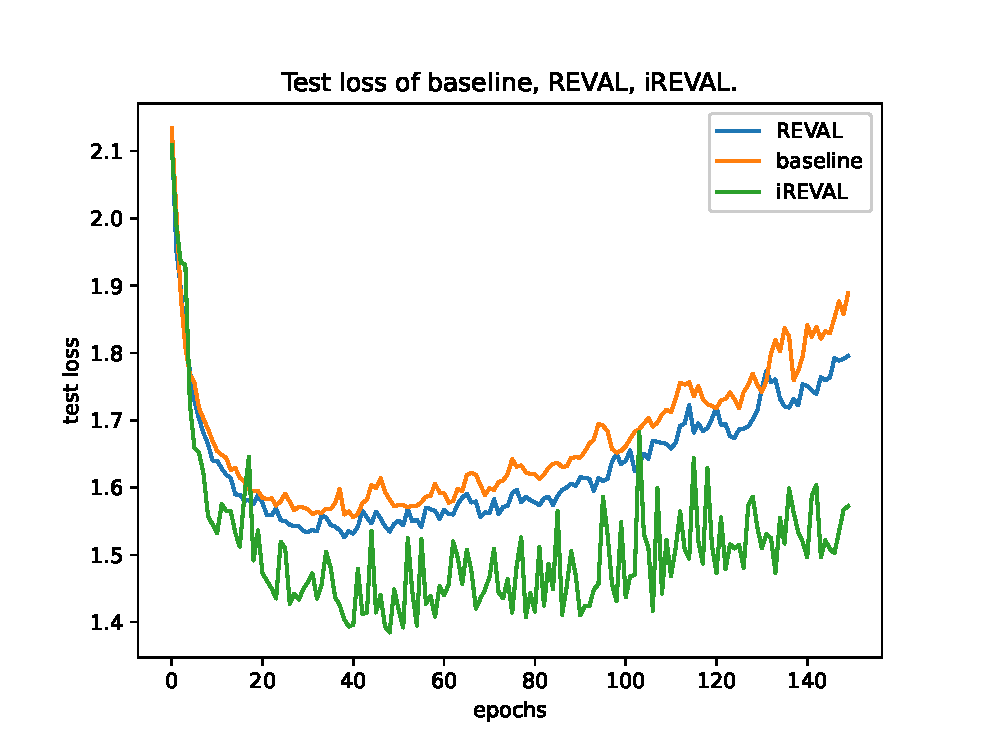
\includegraphics[scale=0.5]{Figures/CIFAR10/test_loss.eps}
    \caption{Test loss of student trained by baseline, REVAL, and iREVAL.}
    \label{fig:test_loss_student}
\end{figure}

The test result on CIFAR-10 is shown in Fig.\ref{fig:test_loss_student} to compare with the baseline, REVAL and iREVAL. The baseline student overfitted after training for 40 epochs. Compared with the baseline, the original REVAL could obtain more generalized solution but still overfitted after the long training. Compared to the previous two methods, iREVAL achieved the lowest test loss and significantly reduced the overfitting problem after the long training. Note that the curve of test loss is not smooth compared to baseline and we consider it is caused by the adversarial objects of students and supervisor.

To show the results in detail, we summarized the train loss and test  accuracy in the Table \ref{table:test_loss_students} and Fig.\ref{fig:CIFAR10_REVAl_Train_LOSS_Test_ACC} to compare the baseline and REVAL. From them we can see, because REVAL and iREVAL obtained lower validation loss and get rid of the overfitting problem, they result in lower train loss and higher test accuracy than the baseline. Compare with REVAL and iREVAL, it shows that the tricks we propose in iREVAL is practical for obtaining more generalized minima.

\begin{figure}[htbp]
\centering
\captionsetup{justification=centering}
\subfigure[]{
    \centering
    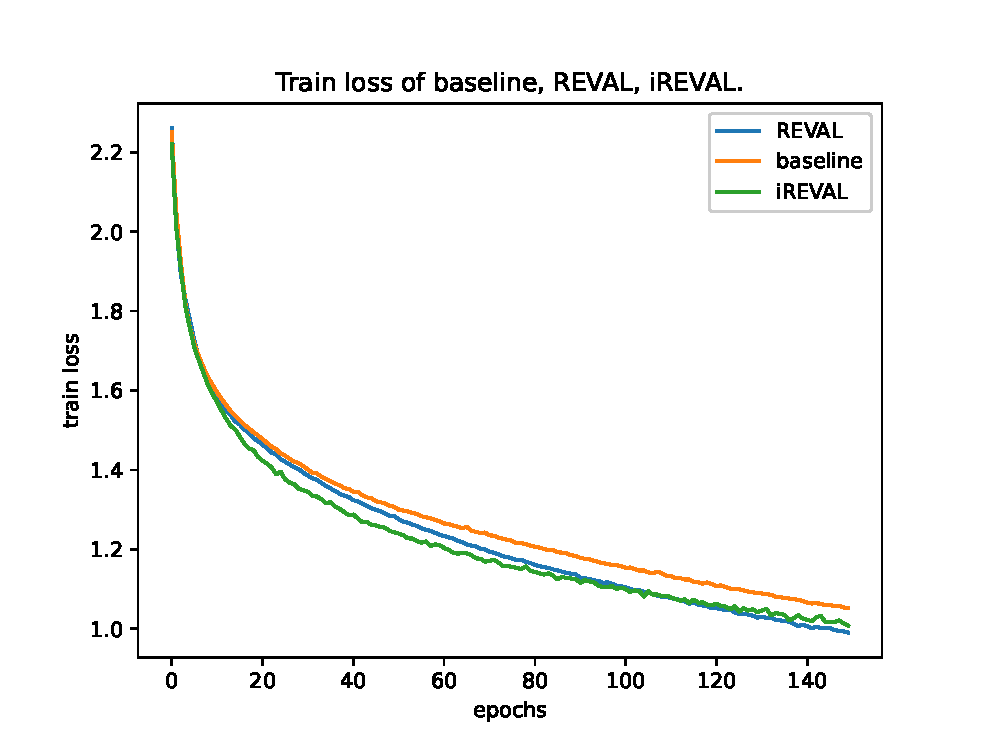
\includegraphics[scale=0.25]{Figures/CIFAR10/train_loss.eps}
}
\subfigure[]{
    \centering
    \includegraphics[scale=0.25]{Figures/CIFAR10/test_metrcis.eps}
}
\caption{Training loss and test accuracy of the baseline, REVAL and iREVAL.}
\label{fig:CIFAR10_REVAl_Train_LOSS_Test_ACC}
\end{figure}

\begin{table}[H]
	\centering
% 	\footnotesize
% 	\setlength{\tabcolsep}{5pt}
	\begin{tabular}{cccc}
		\toprule [1.3pt]	
		\hline
		\multirow{2}{1.1cm}{\centering \textbf{Method}} & \multirow{2}{*}{\textbf{Train loss}} &
		\multirow{2}{*}{\textbf{Test loss}} & \multirow{2}{*}{\textbf{Test accuracy}} \\
		&  &  & \\		
		\hline
		baseline & 1.137 & 1.586 & 43.7\% \\
		\hline
		REVAL &  0.996  & 1.553 &  44.8\%\\
		\hline
		iREVAL &  1.005  & 1.398 & 47.8\%\\
		\hline
		\bottomrule[1.3pt]
	\end{tabular}
	\caption{Comparison of the baseline, REVAL and iREVAL on CIFAR-10 dataset.}
	\label{table:test_loss_students}
\end{table}


\subsubsection{Effectiveness of Supervisor}
In the Fig.\ref{fig:vloss_sloss}, we show how accurate of the supervisor's prediction on student's test loss. In this figure, the blue line is the student's test loss during training. The orange line is the supervisor's prediction from the training weights of student. This figure show us the supervisor could catch the scale and the time steps of the overfitting.

\begin{figure}
    \centering
    \captionsetup{justification=centering}
    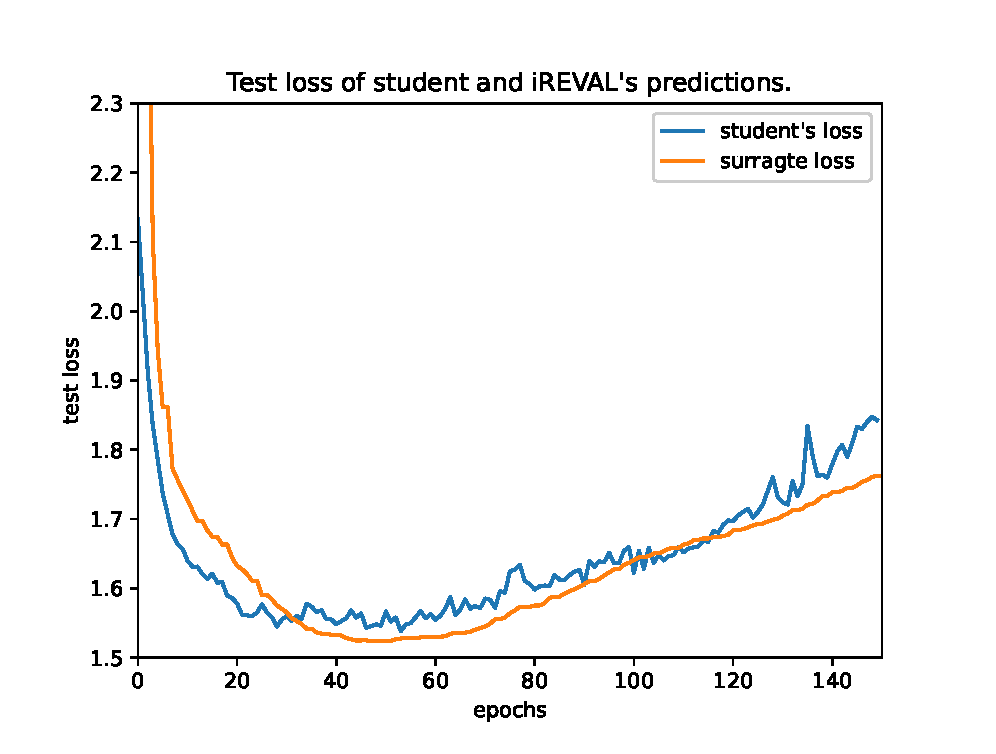
\includegraphics[scale=0.5]{Figures/CIFAR10/sp_st_surrogate_loss.eps}
    \caption{Supervisor's prediction compared to student's test loss.}
    \label{fig:vloss_sloss}
\end{figure}

We show the train loss and test loss of supervisor in Fig.\ref{fig:REVAL_train_test}. In this figure, the orange line is the train loss and the blue line is the test loss. Because we add new students to the dataset when training supervisor, the curve is not smooth. But the train curve still converged fast after $200$ epochs, this means the new student won't add new information about the loss surface to the supervisor. We consider this is the reason why REVAL's training curve is similar to the baseline shown in Fig.\ref{fig:test_loss_student}.

\begin{figure}
    \centering
    \captionsetup{justification=centering}
    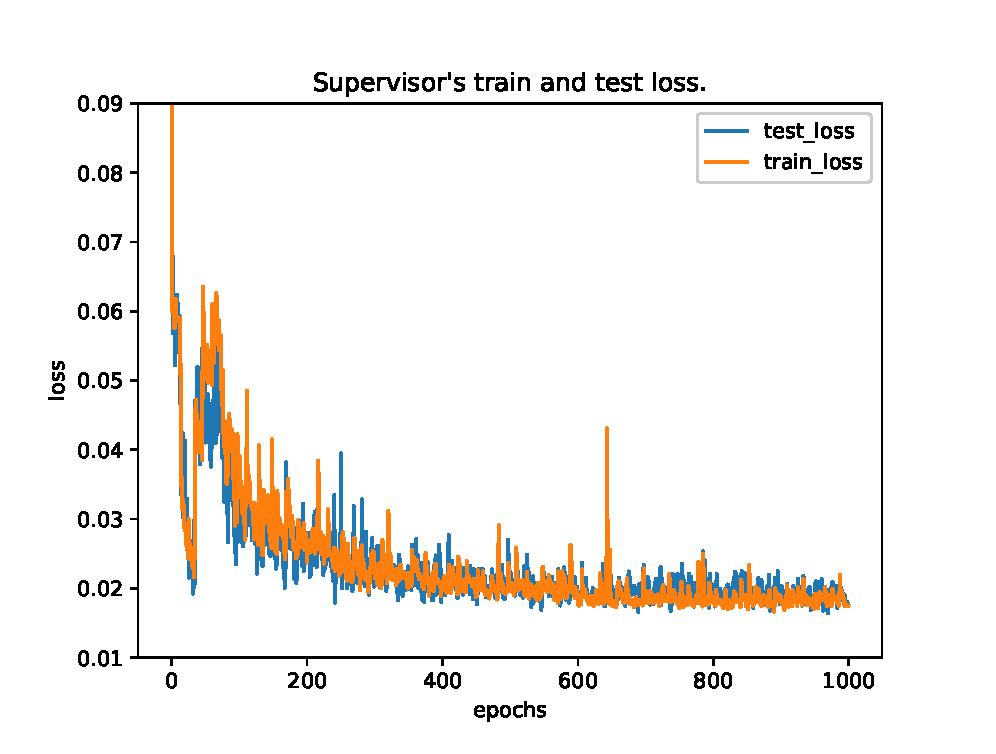
\includegraphics[scale=0.5]{Figures/CIFAR10/sp_train_test.eps}
    \caption{Supervisor's train and test loss in REVAL.}
    \label{fig:REVAL_train_test}
\end{figure}

\subsubsection{Improvments by Tricks}

\begin{figure}
    \centering
    \captionsetup{justification=centering}
    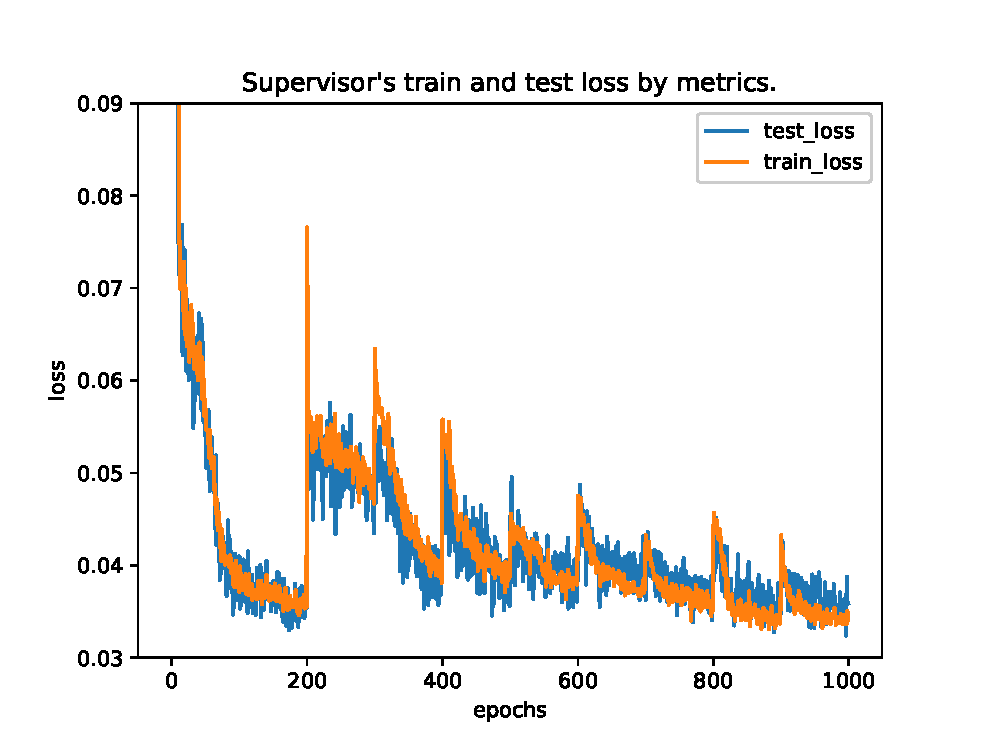
\includegraphics[scale=0.5]{Figures/CIFAR10/sp_ol_train_test.eps}
    \caption{Supervisor's train and test loss in iREVAL.}
    \label{fig:iREVAL_train_test}
\end{figure}

\begin{figure}[htbp]
\centering
\captionsetup{justification=centering}
\subfigure[]{
    \centering
    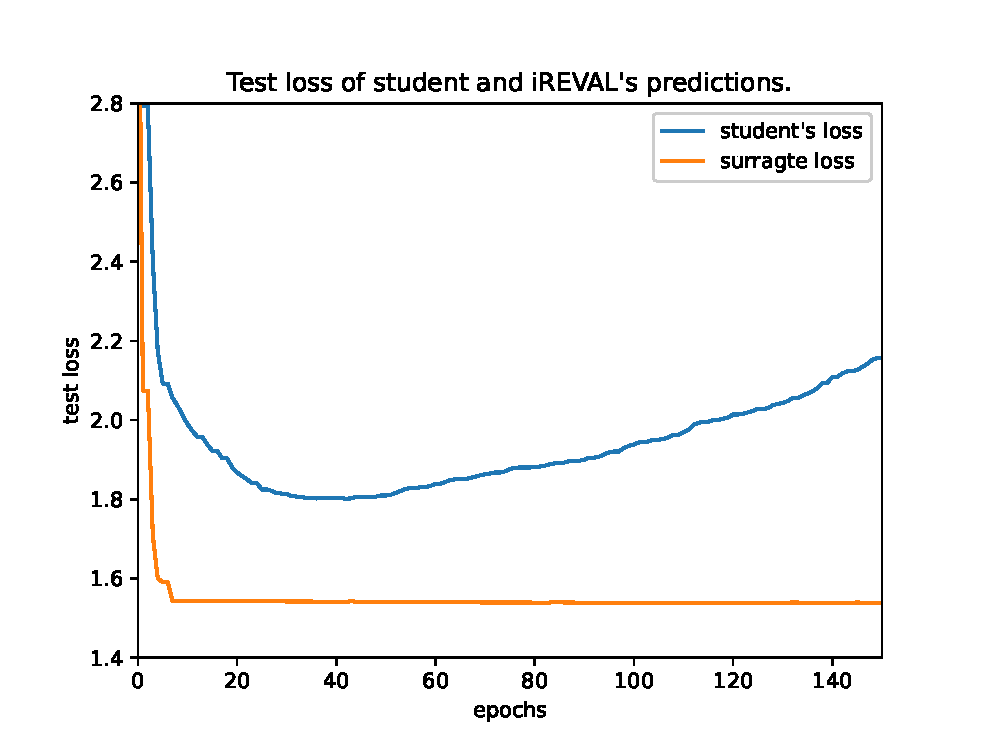
\includegraphics[scale=0.25]{Figures/CIFAR10/sp_surrogate_loss.eps}
}
\subfigure[]{
    \centering
    \includegraphics[scale=0.25]{Figures/CIFAR10/online_surrogate_loss.eps}
}
\caption{Comparison of how the offline and online training effect of supervisor's prediction.}
\label{fig:CIFAR10_REVAl_Supervisor}
\end{figure}

\begin{table}[H]
	\centering
	\begin{tabular}{cccc}
		\toprule [1.3pt]	
		\hline
		\multirow{2}{1.1cm}{\centering \textbf{Method}} & \multirow{2}{*}{\textbf{Train loss}} &
		\multirow{2}{*}{\textbf{Test loss}} & \multirow{2}{*}{\textbf{Params}} \\
		&  &  & \\		
		\hline
		REVAL &  0.996  & 1.553 &  44.8\%\\
		\hline
		iREVAL &  1.005  & 1.398 & 47.8\%\\
		\hline
		\bottomrule[1.3pt]
	\end{tabular}
	\caption{Comparison of the REVAL and iREVAL supervisors on CIFAR-10 students.}
	\label{table:test_loss_supervisor}
\end{table}

\section{Conclusion and Future Work}


\balance

\printbibliography %Prints bibliography

\section*{Appendix}

\end{document}
